\newpage
\section{Iteración 3: Modelo del mapa e interfaz}

\subsection{Introducción}
Durante el desarrollo de la iteración anterior se logró construir y optimizar el robot, integrando compensaciones en el sistema de control para mejorar su estabilidad y precisión operativa.

En la presente iteración se busca avanzar aún más en las capacidades del robot mediante el modelado del espacio en el que operará, esto mediante la creación de una representación del mapa de su entorno.

Además, se buscará desarrollar una interfaz de usuario que facilitará la interacción y monitoreo del sistema.

\subsection{Requerimientos}
En esta iteración abordaremos los siguientes requerimientos funcionales:

\begin{center}
\begin{tabular}{
    | >{\centering\arraybackslash}m{1cm}
    | >{\centering\arraybackslash}m{13cm} |
}
\hline \rowcolor{test_header_color}
    ID & Descripción \\
\hline
    RF7 & Debe existir un modo de calcular trayectorias automáticamente. \\
\hline
    RF10 & Debe existir una interfaz de usuario para control y monitoreo. \\
\hline
\end{tabular}
\end{center}

Por otra parte, los requerimientos no funcionales que trataremos son:

\begin{center}
\begin{tabular}{
    | >{\centering\arraybackslash}m{1cm}
    | >{\centering\arraybackslash}m{13cm} |
}
\hline \rowcolor{test_header_color}
    ID & Descripción \\
\hline
    RNF1 & Debería tener tiempos de respuesta aceptables para el buen funcionamiento del sistema de control. \\
\hline
    RNF2 & El software debería contar con pruebas unitarias y de integración. \\
\hline
    RNF4 & El código debería contar con documentación.\\
\hline
\end{tabular}
\end{center}

\subsection{Desarrollo}

\subsubsection{Modelado del mapa}

Para empezar, es crucial tener un diseño inicial del entorno donde se moverá el robot, que incluya paredes, obstáculos y puntos de interés. Dado que el robot solo se mueve en líneas rectas, este proceso puede ser más sencillo en comparación con robots que tienen libertad de movimiento en todas las direcciones.

El siguiente paso fue la creación del modelo del mapa, donde se divide el entorno en una cuadrícula (grid) y cada celda se marca como libre, ocupada, obstáculo o borde. Cada celda es cuadrada y tiene un lado de $0.5[m]$. Además de ello, el control de movimiento del robot debe estar alineado con los ejes de la grid, y se utilizan algoritmos como A* o Dijkstra para planificar rutas en línea recta.

Mientras el robot se mueve y los sensores recopilan datos, las celdas de la grid se deben actualizar continuamente, indicando si están libres u ocupadas. Esta actualización constante del mapa es esencial para mantener la precisión y eficiencia en el mapeo. Al mismo tiempo, es importante validar que el mapa generado es preciso y coincide con el entorno real.

Debajo se muestra el modelo del mapa que consideramos para el proyecto. Decidimos que los colores de referencia son:

\begin{itemize}
    \item Rojo: borde o límite del mapa
    \item Blanco: obstáculo
    \item Gris: celda ocupable libre
    \item Otro: robot ocupando una celda
\end{itemize}

El punto verde en la imagen de debajo simboliza el origen efectivo del mapa, es la primera celda ocupable del mapa. Además en el centro existe un obstáculo que torna a esa celda no ocupable. Las coordenadas representadas en el mapa son coordenadas ordinales de las celdas, al realizar la odometría se toma el valor de medición en metros. Por lo que si el robot está en la celda $(3, 2)$, la posición reportada por la odometría será $(1.5, 1.0)$, dado que cada celda tiene $0.5[m]$ de lado.

\begin{figure}[H]
    \centering
    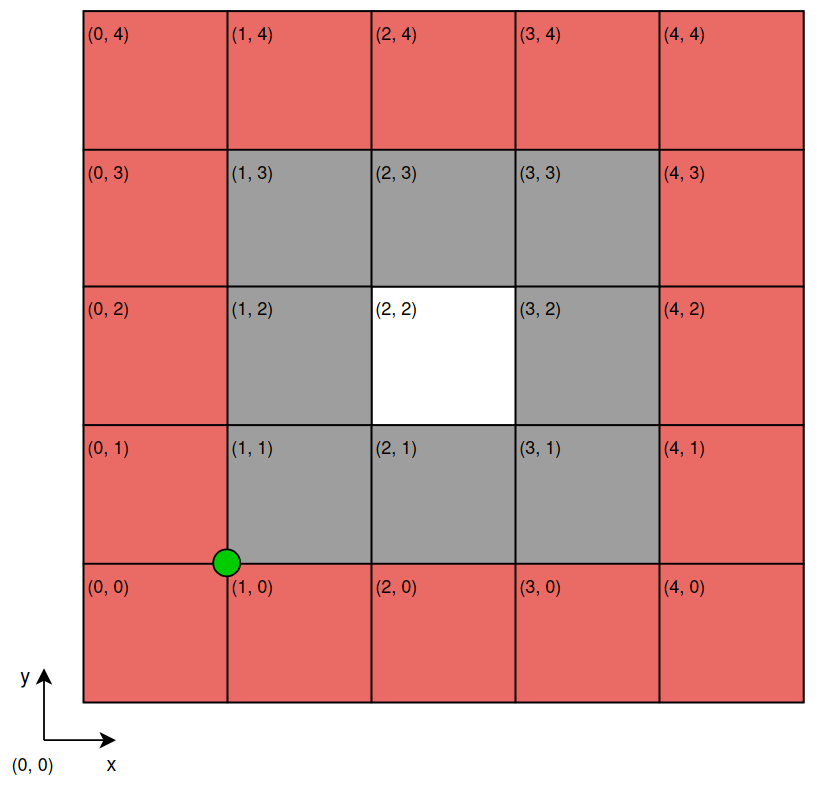
\includegraphics[width=0.8\linewidth]{images/modelo_del_mapa.png}
    \caption{Modelo del mapa}
    \label{fig:modelomapa}
\end{figure}


\subsubsection{Path Finder}

Dentro de los algoritmos de planificación de trayectorias, elegimos utilizar A* por su gran eficiencia en encontrar el camino mas corto y ser ampliamente conocido y estudiada su efectividad. Su objetivo es encontrar el camino más corto entre dos puntos en un mapa combinando las ventajas de los algoritmos de búsqueda de coste uniforme y heurística. \cite{sariffpathplan} \cite{cuevaspathfinding}

$A*$ funciona evaluando cada celda del mapa utilizando una función de costo:

$$ f(n) = g(n) + h(n) $$

Donde $g(n)$ es el costo acumulado desde el punto inicial hasta la celda actual, y $h(n)$ es una heurística que estima el costo restante desde la celda actual hasta el destino. La heurística debe ser admisible, lo que significa que nunca sobreestima el costo real para garantizar que el algoritmo encuentre el camino más corto.

El proceso comienza con la celda inicial, que se agrega a una lista abierta (open list) de celdas por explorar. En cada paso, el algoritmo selecciona la celda con el valor $f(n)$ más bajo de la lista abierta y la mueve a una lista cerrada (closed list) de celdas ya exploradas. Luego, evalúa las celdas vecinas de la celda actual. Si una celda vecina no está en la lista cerrada y no hay una ruta mejor a esa celda en la lista abierta, se actualizan sus valores de $g$, $h$ y $f$, y se agrega a la lista abierta.

Este proceso se repite, seleccionando y evaluando celdas hasta que se alcanza la celda destino. A medida que se avanza, $A*$ construye el camino más corto de regreso desde el destino hasta el origen siguiendo los valores de $g$. La clave del éxito del algoritmo $A*$ es su capacidad para equilibrar de manera eficiente el costo acumulado $g(n)$ y la heurística $h(n)$, permitiéndole encontrar rutas óptimas de manera efectiva.

La eficiencia de $A*$ depende en gran medida de la heurística utilizada. La heurística más común es la distancia de Manhattan para movimientos en una cuadrícula ortogonal, o la distancia euclidiana para movimientos en cualquier dirección. En nuestro caso la técnica mas conveniente es utilizar la distancia de Manhattan.



\subsubsection{Interfaz de usuario}

En la pantalla principal de la interfaz se muestra un mapa interactivo del entorno, con una cuadrícula que representa el mapa. La interfaz muestra información en tiempo real sobre la celda actual en la que se ubica el robot en el mapa, actualizándose conforme el robot se desplaza. Además, se proporciona información sobre la dirección de movimiento.

El usuario comienza estableciendo los puntos de inicio y destino haciendo click en las celdas disponibles. Cuando se da la orden de inicio, se calcula la ruta óptima y se envían los comandos al robot. Paso seguido, la interfaz muestra continuamente en tiempo real la celda del robot y se envían los comandos de movimiento hacia las celdas subsiguientes.

\begin{figure}[H]
    \centering
    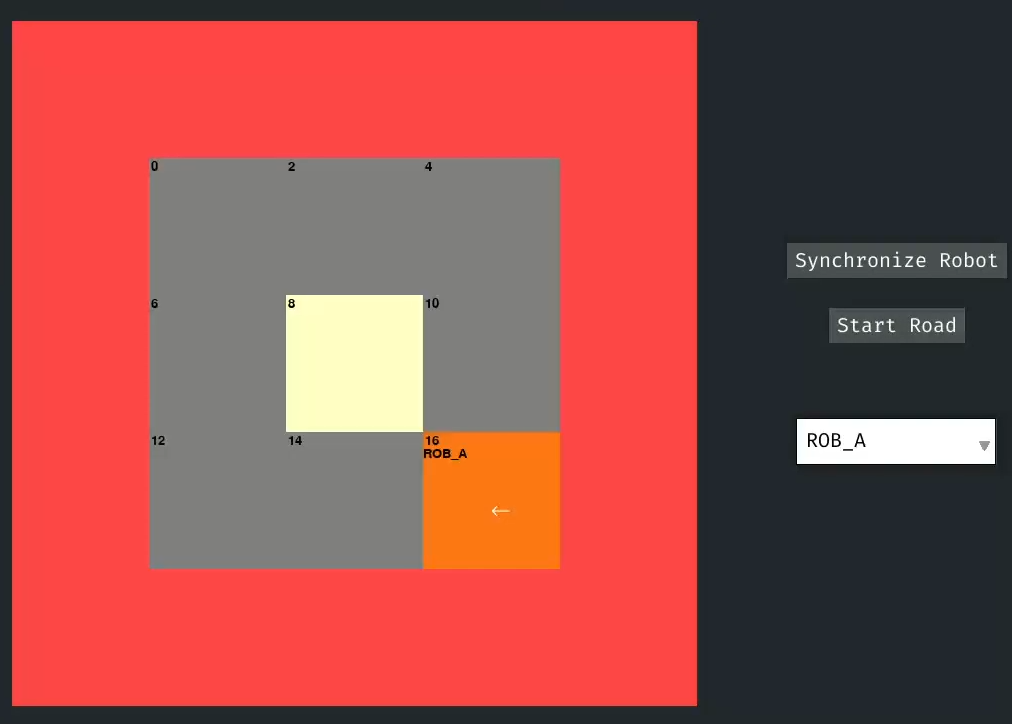
\includegraphics[width=0.85\linewidth]{images/interfaz_de_usuario}
    \caption{Interfaz de usuario}
    \label{fig:interfazusuario}
\end{figure}



\input{iteraciones_desarrollo/iteracion_3/diseño_pista}

\subsection{Testing y pruebas}

\begin{testtableformat}
    \hline \rowcolor{test_header_color}
        Test ID             & TC\_03\_00 \\
    \hline
        Tipo de test        & Test unitario \\
    \hline
        Objeto de prueba    & Calculador de trayectorias \\
    \hline
        Requerimiento       & RF7 \\
    \hline
        Nombre              & Cálculo de trayectorias en un mapa con obstáculos, trayectoria resoluble \\
    \hline
        Descripción         & Calcular la secuencia de coordenadas a seguir para llegar a un punto A a un punto B del mapa, con obstáculos dispuestos de modo que existe al menos una trayectoria posible \\
    \hline
        Precondición        & PRECOND\_E \\
    \hline
        Pasos del test      & \begin{enumerate}
                                \item Enviar al PathFinder una coordenada origen y una destino de modo que exista un camino soluble entre ellas
                                \item Verificar que la salida del PathFinder consiste en la secuencia de coordenadas del mapa que se deben visitar para llegar del origen al destino
                                \item Repetir desde el paso 1) con diferentes valores
                            \end{enumerate} \\
    \hline
        Resultado esperado  & Se obtiene la secuencia adecuada para los puntos dados y se cumple la restricción de solo movimientos horizontales o verticales \\
    \hline
        Resultado obtenido  & La secuencia de coordenadas calculadas se corresponden a las más óptimas para cada par de puntos y se cumple la restricción de movimiento \\
    \hline
        Observaciones       & - \\
    \hline
\end{testtableformat}


\begin{testtableformat}
    \hline \rowcolor{test_header_color}
        Test ID             & TC\_03\_01 \\
    \hline
        Tipo de test        & Test unitario \\
    \hline
        Objeto de prueba    & Calculador de trayectorias \\
    \hline
        Requerimiento       & RF7 \\
    \hline
        Nombre              & Cálculo de trayectorias en un mapa con obstáculos, trayectoria irresoluble \\
    \hline
        Descripción         & Calcular la secuencia de coordenadas a seguir para llegar a un punto A a un punto B del mapa, con obstáculos dispuestos de modo que no existe ninguna trayectoria posible \\
    \hline
        Precondición        & PRECOND\_F \\
    \hline
        Pasos del test      & \begin{enumerate}
                                \item Enviar al PathFinder una coordenada origen y una destino de modo que no exista camino posible entre ellas
                                \item Verificar que la salida del PathFinder es un error
                                \item Repetir desde el paso 1) con diferentes valores
                            \end{enumerate} \\
    \hline
        Resultado esperado  & Se obtiene un mensaje de error informando que no existe trayectoria posible \\
    \hline
        Resultado obtenido  & El error se presenta solo cuando se define el mapa de modo que entre un punto A y un punto B no existe camino posible \\
    \hline
        Observaciones       & - \\
    \hline
\end{testtableformat}


\subsection{Resultados}
Uno de los principales resultados fue el desarrollo de una interfaz de usuario simple que facilita el control y la supervisión del robot. Aparejado con ello, se introdujo un calculador de trayectorias que optimiza los movimientos del robot en el espacio modelado.

Por último se logró implementar una pista fabricada con madera MDF, con imanes integrados, la cual garantiza estabilidad y uniformidad en las pruebas del sistema. Esta pista, además, fue modelada y representada tanto en el mapa desarrollado como en la interfaz, manteniendo la coherencia del entorno del robot.


\begin{figure}[H]
    \centering
    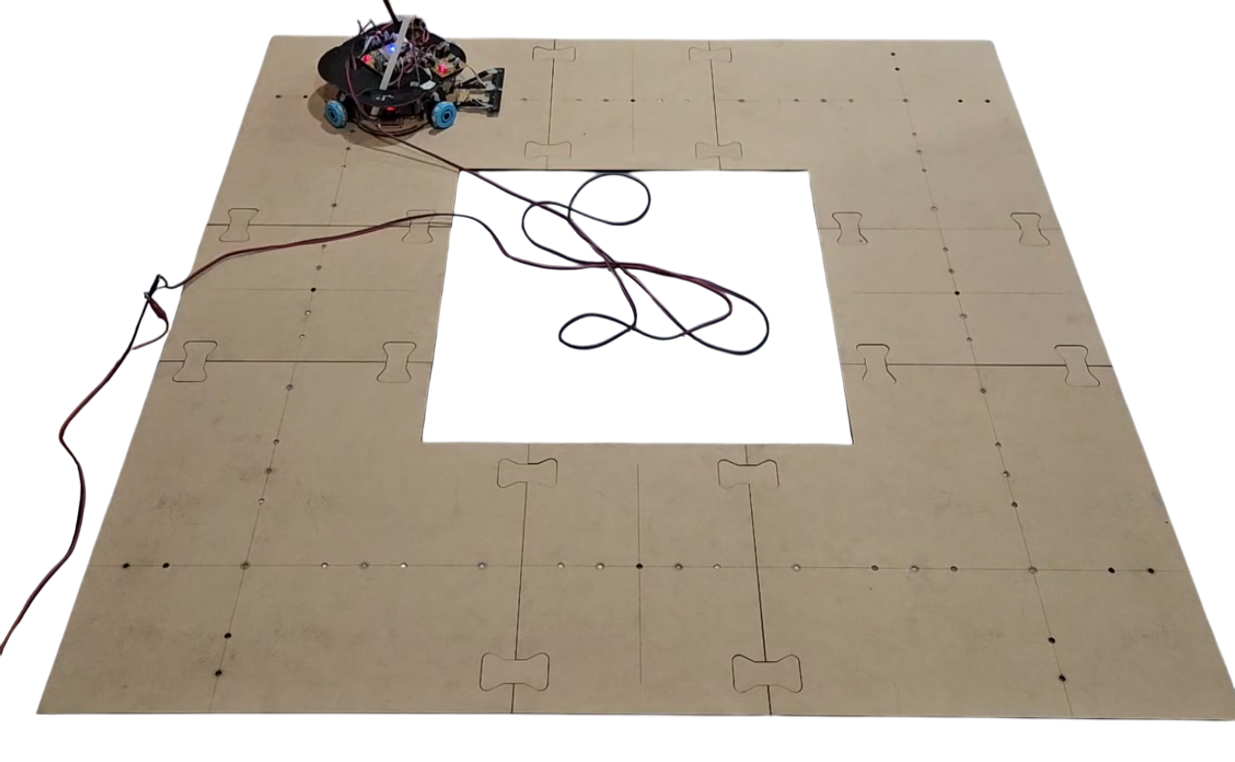
\includegraphics[width=1\linewidth]{images/robot_en_pista_final.png}
    \caption{Robot en la pista con imanes}
    \label{fig:robotpistaconimanes}
\end{figure}

\subsection{Riesgos superados}
En esta iteración pudimos demostrar que los nuevos componentes integrados al sistema interactúan efectivamente con los ya desarrollados en las iteraciones previas, por lo que se avanza sobre el riesgo RI-02.

Del mismo modo, se supera en parte el riesgo RI-05 por tener una alta disponibilidad de servicios de corte láser en MDF y los imanes son muy accesibles.

\begin{center}
\begin{tabular}{|c|c|} 
    \hline \rowcolor{test_header_color}
        ID & Riesgo \\
    \hline
        RI-02 & Intercomunicación de componentes ineficiente o ineficaz \\
    \hline
        RI-05 & Dificultad en conseguir determinados componentes. \\
    \hline
\end{tabular}
\end{center}

\subsection{Conclusiones}

En esta iteración del proyecto se han alcanzado avances fundamentales, como la inclusión de un calculador de trayectorias que optimiza los movimientos del robot dentro de la pista, marcando un avance fundamental para su rendimiento.

Asimismo, se avanzó con la creación de una interfaz de usuario funcional y sencilla permitiendo un control y monitoreo más efectivo del sistema. 

Por su parte, la implementación de una pista de superficie consistente que representa el espacio de movimiento del robot ha proporcionado un entorno operacional estable, ideal para las pruebas del robot.

En definitiva, el proyecto avanza hacia su consolidación como una solución robusta, eficiente y adaptable.